\documentclass[11pt]{article}
\usepackage[margin=1in]{geometry}
\usepackage{amsmath,amssymb,amsthm,mathtools}
\usepackage{graphicx}
\usepackage[hidelinks]{hyperref}
\emergencystretch=3em

\newtheorem{theorem}{Theorem}
\newtheorem{lemma}{Lemma}
\newtheorem{remark}{Remark}

\newcommand{\R}{\mathbb R}
\newcommand{\rank}{\operatorname{rank}}
\newcommand{\dd}{\,\mathrm d}

\title{The One-Dimensional-Kernel Case of the Minor-Invariant Projection Question}
\author{Run fa\_banach\_001, lane 19}
\date{July 19, 2026}

\begin{document}
\maketitle

\section*{Source Question}

Guerra and Raita ask in Question 5.17 of arXiv:1909.03923 for conditions on a
projection
\[
  T:\R^{m\times n}\to V\subseteq \R^{m\times n}
\]
under which one can find a nonzero linear combination $H_s$ of $s$-minors,
$2\le s<\min\{m,n\}$, satisfying
\[
  H_s(X)=H_s(X+Y)
  \quad\text{for every }X\text{ and every }Y\text{ with }T(Y)=0.
\]
Equivalently, $H_s$ is a linear combination of $s$-minors depending only on the
coordinates of $V$. The source passage is shown in Figure~\ref{fig:source}.

\begin{figure}[t]
\centering
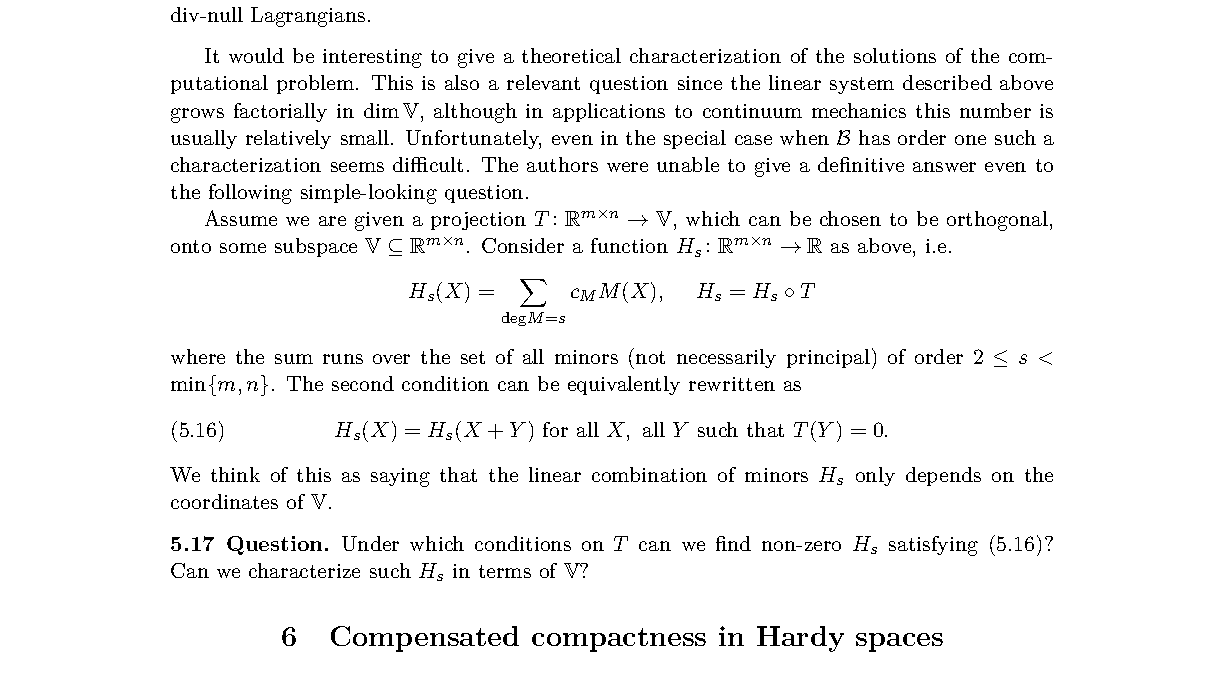
\includegraphics[width=\textwidth,height=.77\textheight,keepaspectratio]{figures/open_question_page.png}
\caption{Question 5.17 in the source paper, printed page 24.}
\label{fig:source}
\end{figure}

This packet gives an exact answer when $\ker T$ is one-dimensional.

\section*{Definitions and Normal Form}

For $I\subset\{1,\dots,m\}$ and $J\subset\{1,\dots,n\}$ with
$|I|=|J|=s$, write
\[
  M_{I,J}(X)=\det X_{I,J},
\]
where $X_{I,J}$ is the submatrix with rows $I$ and columns $J$, both listed in
increasing order. A linear combination of $s$-minors is a polynomial
\[
  H(X)=\sum_{\substack{|I|=s\\ |J|=s}} c_{I,J}M_{I,J}(X).
\]

If $\ker T=\R A$, then the source condition is exactly
\[
  H(X+tA)=H(X)\quad\text{for all }X\in\R^{m\times n},\ t\in\R .
\]
Let $r=\rank A$. By invertible row and column operations there are
$P\in GL_m(\R)$ and $Q\in GL_n(\R)$ such that
\[
  PAQ=D_r,
\]
where $D_r$ is the $m\times n$ matrix with ones in the entries
$(1,1),\dots,(r,r)$ and zeros elsewhere. By the Cauchy-Binet formula,
$X\mapsto K(PXQ)$ and $X\mapsto K(P^{-1}XQ^{-1})$ carry the vector space
spanned by $s$-minors onto itself. Thus the existence of a nonzero invariant
combination for the direction $A$ is equivalent to the same existence problem
for the normal-form direction $D_r$.

\section*{Proof Intuition}

After the reduction to $D_r$, the kernel direction changes only the first $r$
diagonal entries. Call these indices active. A single minor $M_{I,J}$ is
automatically invariant if no active index belongs to both $I$ and $J$, because
then the shifted diagonal entries never occur inside the submatrix. Such
row/column sets exist exactly when two $s$-sets can be placed in the $m$ row
slots and $n$ column slots without double-using any of the $r$ active indices;
this is the counting condition $2s\le m+n-r$.

In the opposite range, every $s$-row set and $s$-column set must share at least
one active index. Differentiating the identity $H(X+tD_r)=H(X)$ gives one
linear equation for each $(s-1)$-minor. The equation for
$M_{I\setminus\{a\},J\setminus\{a\}}$ contains the coefficient of
$M_{I,J}$. If one descends on the number of active indices appearing in
$I\cup J$, the other coefficients in that same equation have already vanished,
so $c_{I,J}$ is isolated and must be zero.

\section*{Main Partial Theorem}

\begin{theorem}[One-dimensional-kernel rank threshold]
\label{thm:main}
Let $m,n\ge 2$, let $2\le s<\min\{m,n\}$, and let
$T:\R^{m\times n}\to V$ be a linear projection with one-dimensional kernel
$\ker T=\R A$, where $A\ne0$ has rank $r$. Then there is a nonzero linear
combination $H$ of $s$-minors satisfying
\[
  H(X)=H(X+Y)\quad\text{whenever }T(Y)=0
\]
if and only if
\[
  2s\le m+n-r.
\]
\end{theorem}

\begin{proof}
By the normal-form discussion above, it is enough to prove the theorem for
$A=D_r$. Write
\[
  R=\{1,\dots,r\}
\]
for the active indices.

First assume $2s\le m+n-r$. This inequality says that it is possible to choose
subsets $I\subset\{1,\dots,m\}$ and $J\subset\{1,\dots,n\}$ with
$|I|=|J|=s$ and
\[
  I\cap J\cap R=\varnothing.
\]
Indeed, choose $I$ with as few active indices as possible. Then
\[
  |I\cap R|=\max\{0,s-(m-r)\}.
\]
If $s\le m-r$, all active column labels remain available and there is no
obstruction to choosing $J$. If $s>m-r$, the number of column labels not
forbidden by $I\cap R$ is
\[
  n-|I\cap R|=n-s+m-r,
\]
which is at least $s$ precisely because $2s\le m+n-r$. Thus such $I,J$ exist.
For such $I,J$, adding $tD_r$ changes only entries $(a,a)$ with $a\in R$, and
none of these entries lies in the submatrix $X_{I,J}$. Hence
$M_{I,J}(X+tD_r)=M_{I,J}(X)$ for all $X,t$, giving a nonzero invariant
$s$-minor.

Conversely, assume $2s>m+n-r$. Then every pair of subsets
$I\subset\{1,\dots,m\}$ and $J\subset\{1,\dots,n\}$ with $|I|=|J|=s$ satisfies
\[
  I\cap J\cap R\ne\varnothing.
\]
Let
\[
  H(X)=\sum_{\substack{|I|=s\\ |J|=s}}c_{I,J}M_{I,J}(X)
\]
be invariant under $X\mapsto X+tD_r$. Differentiating at $t=0$ gives the
polynomial identity
\[
  0=\left.\frac{\dd}{\dd t}\right|_{t=0}H(X+tD_r).
\]
For one minor,
\[
  \left.\frac{\dd}{\dd t}\right|_{t=0}M_{I,J}(X+tD_r)
  =
  \sum_{a\in I\cap J\cap R}
  \varepsilon(a;I,J)\,M_{I\setminus\{a\},J\setminus\{a\}}(X),
\]
where each $\varepsilon(a;I,J)$ is $1$ or $-1$.

The minors of a fixed order are linearly independent as polynomials: every
monomial in $M_{I,J}$ uses exactly the row set $I$ and the column set $J$.
Therefore, for every pair $I_0,J_0$ of $(s-1)$-subsets, the coefficient of
$M_{I_0,J_0}$ in the differentiated identity is zero:
\[
  \sum_{a\in R\setminus (I_0\cup J_0)}
  \varepsilon(a;I_0\cup\{a\},J_0\cup\{a\})
  c_{I_0\cup\{a\},J_0\cup\{a\}}=0.
  \tag{1}
\]
Here $I_0\cup J_0$ is understood as a union of active labels when intersected
with $R$; equivalently the condition on $a$ is $a\notin I_0$ and $a\notin J_0$.

We now prove that all coefficients vanish by descending induction on
\[
  N(I,J)=|(I\cup J)\cap R|.
\]
The largest possible value is $r$. Suppose first that $N(I,J)=r$. Choose
$a\in I\cap J\cap R$ and set $I_0=I\setminus\{a\}$,
$J_0=J\setminus\{a\}$. Since $(I\cup J)\cap R=R$, we have
\[
  R\setminus (I_0\cup J_0)=\{a\}.
\]
Thus equation (1) contains only the term
$\varepsilon(a;I,J)c_{I,J}$, so $c_{I,J}=0$.

Now fix $N<r$ and assume all coefficients $c_{I',J'}$ with
$N(I',J')>N$ have already been shown to vanish. Take $I,J$ with
$N(I,J)=N$. Choose $a\in I\cap J\cap R$ and again set
$I_0=I\setminus\{a\}$, $J_0=J\setminus\{a\}$. In equation (1), the summand
with added index $a$ is precisely $\varepsilon(a;I,J)c_{I,J}$. Any other
summand has added index $b\in R\setminus((I\cup J)\cap R)$, so
\[
  N(I_0\cup\{b\},J_0\cup\{b\})=N+1.
\]
Its coefficient is zero by the induction hypothesis. Equation (1) therefore
reduces to $\varepsilon(a;I,J)c_{I,J}=0$, and hence $c_{I,J}=0$.

Since every $I,J$ in the range $2s>m+n-r$ has a common active index, the
descending induction applies to every coefficient. Hence $H=0$. This proves
that no nonzero invariant combination exists in the opposite range.
\end{proof}

\section*{Relation to the Earlier Trace-Free Packet}

The previous packet
\[
\texttt{1909.03923\_tracefree\_minor\_invariant\_threshold}
\]
handled the square trace-free projection, where $\ker T=\R I_n$. In the
notation of Theorem~\ref{thm:main}, this has $m=n$ and $r=n$, so the threshold
becomes $2s\le n$. Thus the present result strictly subsumes that slice while
still remaining a partial answer to the full Question 5.17.

\section*{Scope and Novelty Check}

The theorem gives an exact existence classification for all projections with
one-dimensional kernel. It does not classify projections whose kernel has
dimension at least two. In the positive range, it proves existence but does not
compute the full invariant subspace.

Cheap run indexes were searched for arXiv:1909.03923, trace-free,
scalar-shift, one-dimensional kernel, rank threshold, minor invariant, and the
source question keywords. The only duplicate-adjacent hit was the earlier
trace-free packet, which is subsumed here. A bounded web search on
July 19, 2026 found the source paper and preprint records but no exact answer
to this one-dimensional-kernel classification.

\section*{Computational Sanity Check}

The script \texttt{code/check\_onedim\_kernel\_threshold.py} constructs the
exact rational matrix of the $D_r$-directional derivative on $s$-minors and
checks the dimension of its kernel for all $3\le m,n\le6$, all
$2\le s<\min\{m,n\}$, and all $1\le r\le\min\{m,n\}$. It verifies that the
kernel is nonzero exactly in the range $2s\le m+n-r$. This computation is only
a sanity check; the proof above is independent.

\section*{References}

\begin{enumerate}
\item A. Guerra and B. Raita,
\emph{Quasiconvexity, null Lagrangians, and Hardy space integrability under
constant rank constraints}, arXiv:1909.03923; Archive for Rational Mechanics
and Analysis 245 (2022), 279--320.
\end{enumerate}

\end{document}
